\documentclass[12pt,a4paper]{article}
\usepackage[utf8]{inputenc}
\usepackage[spanish]{babel}
\usepackage{amsmath}
\usepackage{amsfonts}
\usepackage{amssymb}
\usepackage{makeidx}
\usepackage{graphicx}
\usepackage{wrapfig}
\usepackage{float}
\usepackage[font=small]{caption, subcaption}
%\usepackage[rflt]{floatflt}
\usepackage[left=2cm,right=2cm,top=2cm,bottom=2cm]{geometry}
\usepackage{enumitem}
\author{Camila Chediack Ciminari}
\date{\today}
\title{Redes Neuronales 2021: Trabajo Práctico N°1}
\begin{document}

\begin{titlepage}

\centering

\includegraphics[scale=0.3]{UNC.PNG}

\vspace{1cm}
{\bfseries\LARGE Universidad Nacional de Córdoba \par}
\vspace{1cm}
{\scshape\Large Facultad de Matemática, Astronomía, Física y Computación\par}
\vspace{1cm}
{\scshape\Huge Trabajo Práctico N°1 de Redes Neuronales}
\vspace{1cm}

{\Large Chediack Ciminari, Camila }
\vspace*{0.3cm}


DNI: 41919762 \\


\vspace*{0.3cm}

E-mail:camila.chediack.c@mi.unc.edu.ar

\end{titlepage}
\begin{center}
\textbf{Primera parte}
\end{center}

Considerando el modelo Integrate-and-Fire para la evolución termporal del potencial de membrana entre el interior y el exterior de una neurona genérica, la ecuación diferencial del modelo \textbf{sin activar el mecanismo de disparo}:

\begin{equation}
\dfrac{dV_m(t)}{dt} = \dfrac{1}{\tau_m}(E_L-V_m(t)+R_m I_e(t))
\end{equation}

a) Considerando a $I_e=0$ la ecuación diferencial a considerar resulta: 

$$\dfrac{dV_m(t)}{dt} = \dfrac{1}{\tau_m}(E_L-V_m(t))$$

Donde en tiempos largos, es decir $t \rightarrow \infty$, dado que la neurona no recibe ningún estímulo o input esta se va a encontrar en su potencial de reposo. 

$$\dfrac{dV_m(t)}{dt} = 0 \rightarrow V_m(t) = E_L$$

\begin{wrapfigure}[27]{l}{10cm}
    \begin{minipage}{\linewidth}
    \centering\captionsetup[subfigure]{justification=centering}
    \subcaption*{\textbf{Gráfico N°1}}
    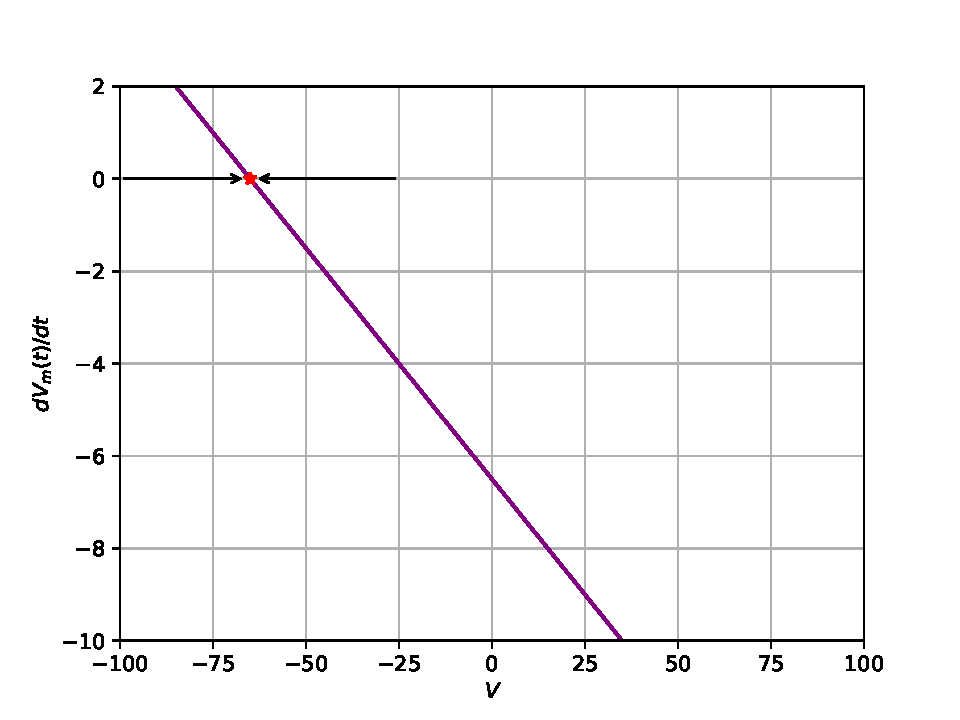
\includegraphics[width=10cm]{PuntoA.pdf}
    \label{PuntoA.pdf}\par\vfill
    \subcaption*{\textbf{Gráfico N°2}}
    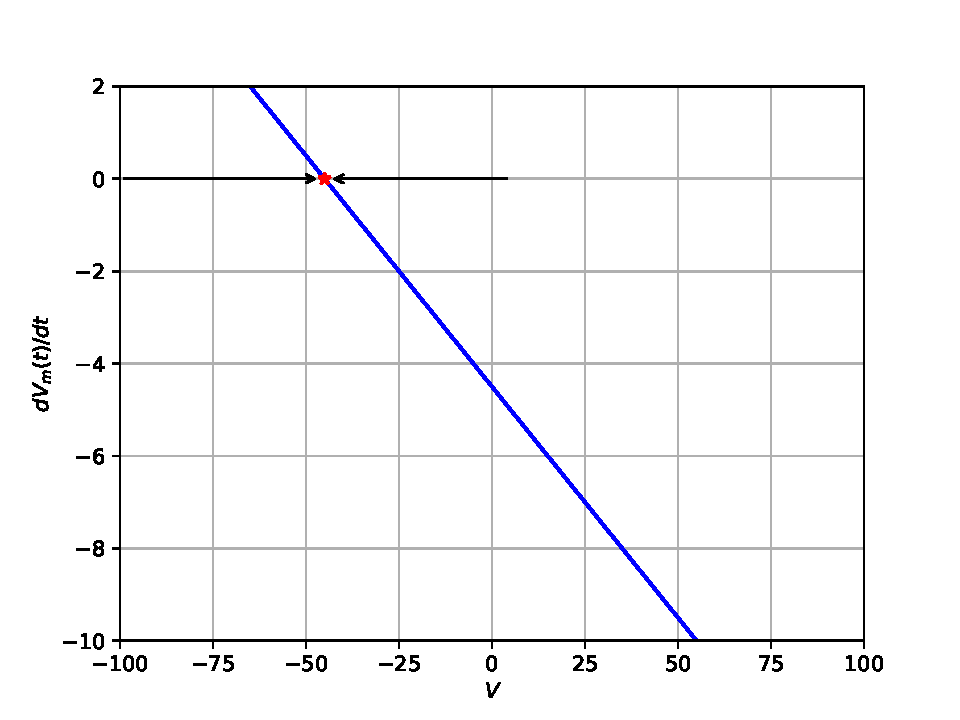
\includegraphics[width=10cm]{PuntoB.pdf}
    \label{PuntoB.pdf}
\end{minipage}
\end{wrapfigure}

La gráfica se puede apreciar en la \textbf{Gráfico N°1}, es una línea recta con pendiente negativa igual a $-1/\tau_m$ donde $\tau_m = 10ms$. Considerando los datos numéricos del problema, el punto fijo se encuentra en las coordenadas $(-65,0)$, el mismo se trata de un punto estable o atractor, cualquier punto inicial que yo elija va a ser atraído por dicho punto. Esto lo podemos corroborar calculando la derivada de la función en dicho punto y ver que esta resulta negativa e igual a $-1/\tau_m$.
\bigskip

b) Considerando el caso en que $I_e = 2nA$, hay un estímulo o input que hace que mi neurona deje de estar en su potencial de reposo ocurriendo una despolarización. 

\begin{align*}
\dfrac{dV_m(t)}{dt}&= (-65mV-V_m(t)+\underbrace{10M\Omega*2nA}_{20mV})\\
&= -45mV - V_m(t)
\end{align*}

Esta situación se representa en la \textbf{Gráfico N°2}, para $t\rightarrow \infty$ el punto fijo, que sigue siendo estable, ahora se encuentra en $(-45, 0)$.
\newpage
c) De forma analítica para un valor arbitrario y constante $I_e(t)=I$ y realizando un cambio de variable, $U(t)= V_m(t)-E_L$.

Diferenciando con respecto a $t$ obtengo $\dfrac{U(t)}{dt} = \dfrac{V_m(t)}{dt}-\underbrace{\dfrac{E_L}{dt}}_{=0} \rightarrow \boxed{\dfrac{U(t)}{dt} = \dfrac{V_m(t)}{dt}}$

Realizando la separación de variables el términos de $U(t)$ e integrando: 
\begin{align*}
\dfrac{U(t)}{dt} &= -\dfrac{1}{\tau_m}(U(t)-R_mI) \\
dt &= -\tau_m \dfrac{dU(t)}{(U(t)-R_mI)} \\
\int{dt} &= -\tau_m \int{\dfrac{dU(t)}{(U(t)-R_mI)}} \\
t &= -\tau_m \ ln(U(t)-R_mI) + C
\end{align*}
Evaluando la constante $C$ en $V(t=0)=V_0$, $C=-ln(U_0-R_mI)$, reemplazando en la ecuación anterior y aplicando propiedad de diferencia de logaritmos:
$$t = -\tau_m \ ln\left( \dfrac{U(t)-R_mI}{U_0-R_mI}\right)$$
Despejando $U(t)$:
$$U(t) = \exp^{-t/ \tau_m}(U_0 - R_mI)+R_mI$$
Ahora reemplazando la variable $U(t)=V(t)-E_L$ obtenemos la expresión analítica de la ecuación diferencial:
$$V(t)=\exp^{-t/ \tau_m}(V_0-E_L-R_mI)+R_mI+E_L$$

\begin{wrapfigure}[15]{r}{10cm}
\caption*{\textbf{Gráfico N°3}}
\label{Sol-exacta-rk4.pdf}
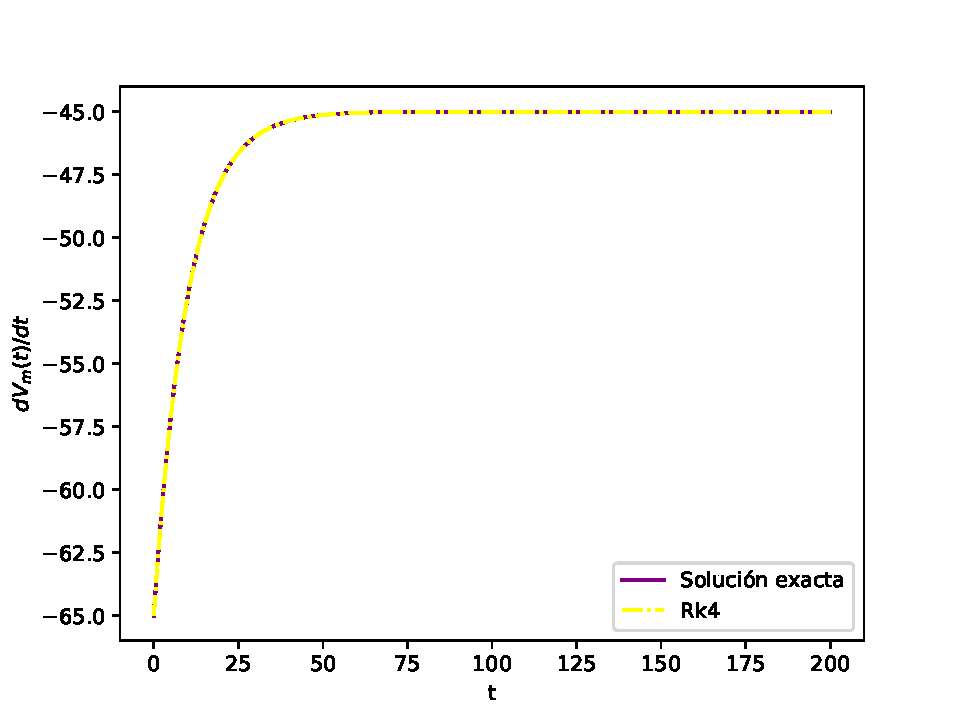
\includegraphics[width=10cm]{Sol-exacta-rk4.pdf}
\end{wrapfigure}

d) En el \textbf{Gráfico N°3} se encuentra la gráfica de la solución exacta representada por la linea continua violeta, se toma la función que se obtuvo en el punto anterior con los valores determinados de los parámetros para $0 ms <t<200ms$.
\bigskip

e) En el \textbf{Gráfico N°3} también se presenta  la aproximación numérica con el método de Runge-Kutta de cuarto orden. Volviendo a la ecuación diferencial (1) se toma $f(V_m,t)$ para encontrar una única trayectoria dentro de las infitas posibles.
\bigskip

\begin{center}
\textbf{Segunda Parte}
\end{center}

f) Al activar el mecanismo de disparo, el potencial de membrana va a superar el umbral $V_{um}=-50 mV$ para un $I_e \geq \dfrac{V_{um}-E_L}{R_m}$. En este caso, manteniendo este estímulo de forma constante, los disparos se van a producir con una cierta frecuencia dado que al pasar el umbral la neurona vuelve a su potencial de reposo. Para que esto último suceda $I_e \geq 1.5nA$, los datos iniciales del problema determinan que este es igual a $2nA$, por lo que se va a generar este estímulo constante que genera una gráfica como la que se ve en el \textbf{Gráfico N°4}. 
\newpage

\begin{figure}[h]
\centering
\caption*{\textbf{Gráfico N°4}}
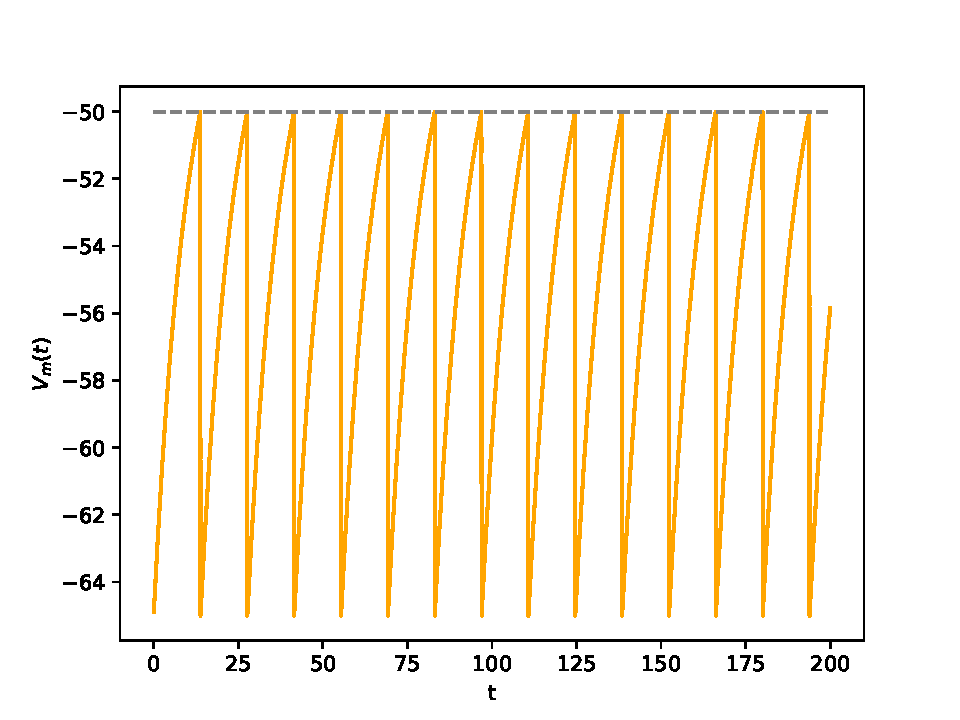
\includegraphics[scale=0.65]{PuntoF.pdf}
\label{PuntoF}
\end{figure}

g) Con $I_e(t)=2.5*cos(t/30)$ el gráfico del punto anterior se ve en el \textbf{Gráfico N°5}. Ahora la corriente eléctrica externa depende del tiempo y se puede notar en el gráfico que la función $cos(t/30)$ provoca una mayor cantidad de oscilaciones, es decir, que los disparos se producen en una menor cantidad de tiempo medido en \textit{ms}.

\begin{figure}[h]
\centering
\caption*{\textbf{Gráfico N°5}}
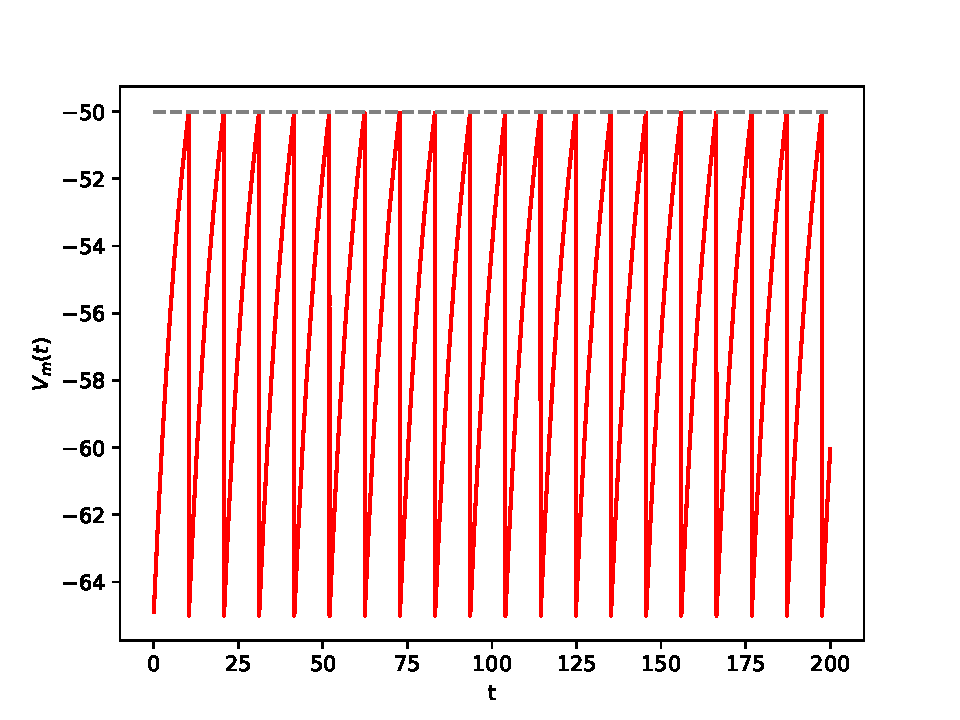
\includegraphics[scale=0.65]{PuntoG.pdf}
\label{PuntoG}
\end{figure}

h) Como se mencionó anteriormente, el disparo sucede con una cierta frecuencia cuando este es lo suficientemente grande como para que el potencial de membrana pase el umbral. Por lo tanto, para obtener la frecuencia de ese disparo se parte de la expresión analítica que iguala el umbral ($V_{um}$) con $V(t)$ cuando esta en reposo $V(t=0)=E_L$.
\setcounter{equation}{0}
\begin{align}
V_{um} &= \exp^{-t/ \tau_m}(\underbrace{V_0-E_L}_{=0}-R_mI)+R_mI+E_L \\
&=\exp^{-t/ \tau_m}(-R_mI)+R_mI+E_L
\end{align}
Despejando $t$ de (2) para obtener el tiempo que tarda la neurona en volver a su potencial de reposo:
\begin{equation}
t = -\tau_m \left[ln\left(1+\dfrac{E_L-V_{um}}{I_e R_m}\right)\right]
\end{equation}
Ahora resta calcular la frecuencia de este disparo, que no es más que la inversa de la ecuación (3). 
\begin{equation}
f = t^{-1} = \left[-\tau_m \ ln\left(1+\dfrac{E_L-V_{um}}{I_e R_m}\right)\right]^{-1}
\end{equation}
\begin{wrapfigure}[15]{r}{9cm}
\caption*{\textbf{Gráfico N°6}}
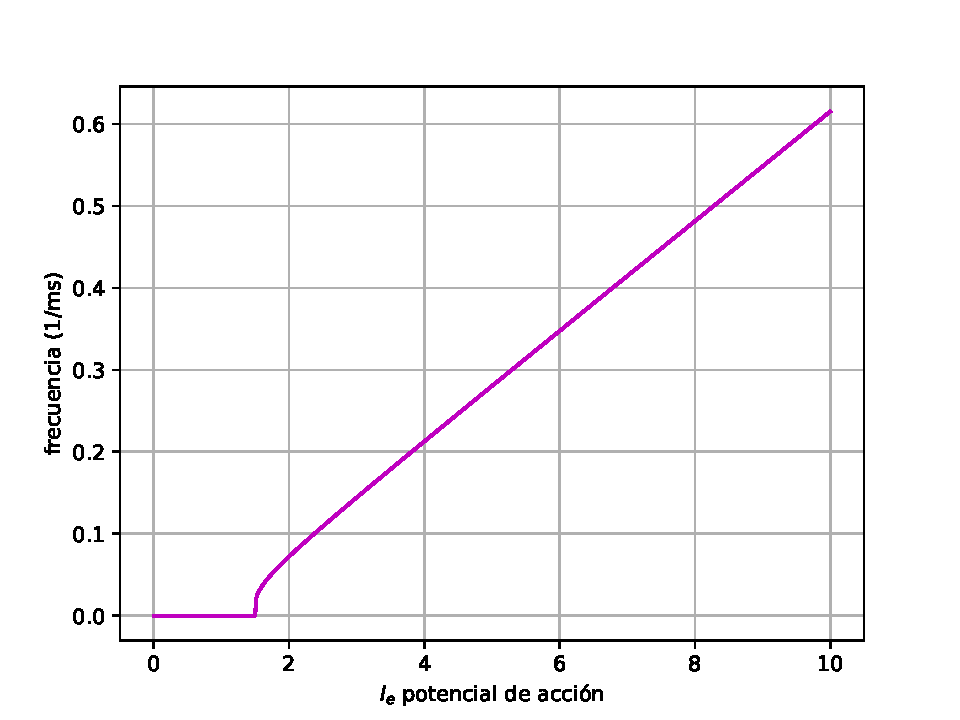
\includegraphics[width=9cm]{frec.pdf}
\label{frec}
\end{wrapfigure}
Reemplazando todas las variables por sus correspondientes valores, con un potencial de acción $I_e=2nA$ (constante), obtenemos que $f\approx0.0721347520$. En la figura de la derecha se encuentra la gráfica de la frecuencia para distintos valores constantes de $I_e$, a partir del punto $1.5$ la función tiene pendiente infinita pero a medida que $I_e$ se aleja de ese valor se vuelve una recta con pendiente positiva.
\bigskip

En la solución numérica del punto F los resultados indican que para un $t=13.850000000000062$ el potencial de membrana paso el umbral y volvio a su potencial de reposo, dado que la frecuencia es la inversa de ese número $f^*= 0.07220216606498163$, cuyo resultado se aproxima bastante bien al obtenido con la ecuación (4). 
\bigskip

i) Se repite el punto f) para un $I_e=0.35(cos(t/3)+sin(t/5)+cos(t/7)+sin(t/11)+cos(t/13))^2$ la función va a mostrar que para algunos momentos el potencial de membrana no llega al umbral, esto se debe a que en esos momentos la corriente eléctrica externa no genera un impulso lo suficientemente grande para alcanzarlo.

\begin{figure}[h]
\centering
\caption*{\textbf{Gráfico N°7}}
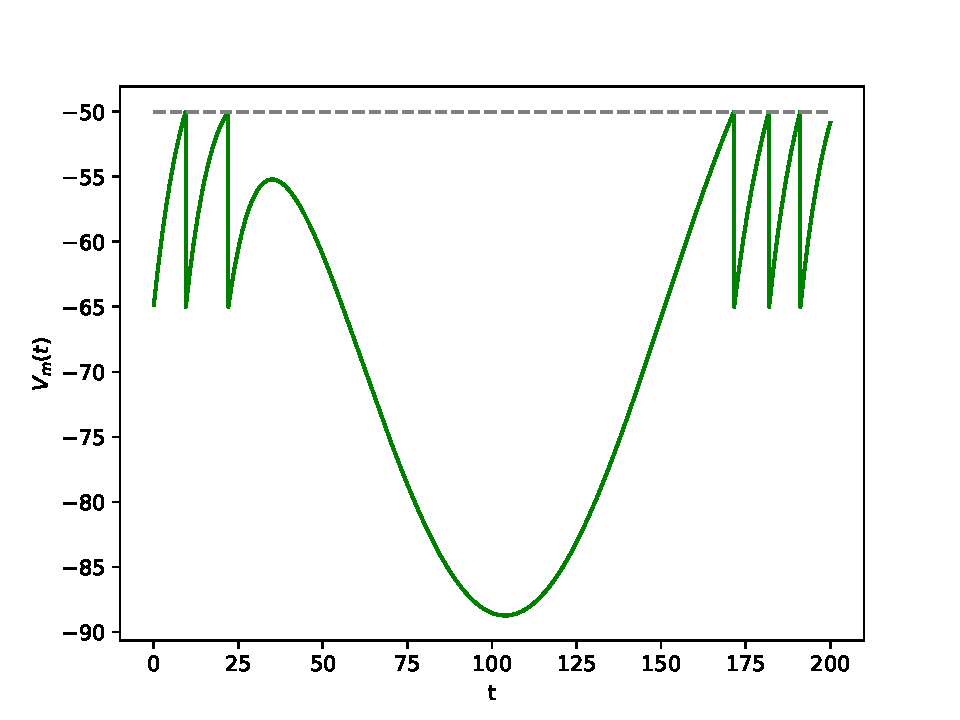
\includegraphics[scale=0.65]{PuntoI.pdf}
\label{PuntoI}
\end{figure}

\end{document}